% Provenance (never printed): see sources/outline_sources.md (Year 2: field and laboratory methods ---
% igneous and metamorphic petrography, chemical analysis by XRF, ICP-MS and microprobe, isotope mass
% spectrometry, a mapping campaign). Modelled on Book 3 ch. 6.
% Textures: BGS RR 99-02 (Robertson 1999), Open University Virtual Microscope, Carleton BH250,
% UCSB Geology 102C (Hacker); QAPF: BGS RR 99-06 (Gillespie and Styles 1999); instruments: SERC
% Geochemical Instrumentation and Analysis sheets (EPMA, WDS, XRF, TIMS, MC-ICPMS); XRF procedure
% and reference-material results: USGS OFR 02-223 and its chapter T (Taggart and Siems 2002); Sr
% isotopes: CIAAW; spike and mass bias: Cheong, Jeong and Kwon (2014). Ledger rows in
% sources/ledger/book4.md; curves and stations from figdata/bachelor-2/labmethods.py, numbers from
% the Book 4 second-writer scratch calculator calc/ch31.py. Observation only: the professional work
% is described in the third person.
\chapter{طرائق الحقل والمختبر II}\label{ch:b2:field-lab-methods-2}

كلّ رقم في فصول علم الصخور في هذا الكتاب بدأ صخرةً في كيس، وشريحةً رقيقة تحت
المجهر، ومسحوقًا في جهاز. فتركيب معدن مرسوم على مخطّط أطوار، ومحتوى
السيليكا الذي يسمّي حمَمًا، ونسبة نظائر السترونشيوم التي تقتفي مصدرًا وشاحيًا: كلّ منها
خرج من سلسلة عمليات بدأت عند مكشف، ويحمل كلّ منها أخطاء كلّ
حلقة فيها. ويتتبّع هذا الفصل تلك السلسلة لصخور قاعدة تلال فاردن: قراءة الأنسجة
في الشريحة الرقيقة، وعدّ المعادن، وتحليل الصخر كاملًا، ثم المعادن المفردة، ثم النظائر،
والتساؤل في كلّ خطوة عن جودة الرقم.

\begin{recall}
\textbf{من مجلّد السنة الأولى}: المحطّة الحقلية، ودفتر الحقل، والعيّنة الموجّهة، والشريحة الرقيقة،
والمجهر المستقطِب، والضوء المستقطَب المستوي، والمستقطِبان المتقاطعان؛ والتعرّف البصري على
المعادن المكوّنة للصخور؛ وإعادة حساب الصيغة المعدنية من تحليل الأكاسيد على عدد ثابت من ذرّات الأكسجين،
وحساب الحديد الثلاثي بتوازن الشحنة؛ والتورّق والشستوزية؛ وخطّ التساوي الزمني، والنسبة الابتدائية وخطّ
المربّعات الصغرى. \textbf{من كتب الكيمياء}: مطيافية الكتلة، والبلازما المقترنة حثّيًا؛
ومنحنى المعايرة، وحدّ الكشف، وحدّ التقدير الكمّي، والدقّة، والصحّة، والانحياز،
والتكرارية، والانحراف المعياري للمتوسّط. \textbf{من كتب الفيزياء}: الأشعة السينية المميِّزة
وقانون موزلي؛ وقانون براغ؛ والتوتّر السطحي؛ وانتشار الارتيابات.
\textbf{من كتب الرياضيات}: التوزيع الحدّاني، ومتوسّطه وتباينه.
\textbf{من \cref{ch:b2:magmatic-series}}: \omterm{def:b2:magmatic-series:qapf}{التركيب المعدني النمطي}، \omterm{def:b2:magmatic-series:qapf}{ومخطّط QAPF}.
\textbf{من \cref{ch:b2:isotope-geochemistry}}: \omterm{def:b2:isotope-geochemistry:tracer}{المقتفي النظائري المشعّ المنشأ}، \omterm{def:b2:isotope-geochemistry:standards}{والمعيار النظائري المرجعي}.
\end{recall}

\section{علم الصخور الوصفي: الأنسجة بوصفها تاريخًا}\label{sec:b2:field-lab-methods-2:petrography}

استعمل مجلّد السنة الأولى المجهر المستقطِب للتعرّف على المعادن. لكنّ عالم الصخور يقرأ أيضًا
كيف ترتّبت الحبيبات، لأنّ الترتيب يسجّل الترتيب الذي نمت به. ونسيجان هما
أشيع الشواهد على التبلور من صهارة وعلى إعادة التبلور في
الحالة الصلبة.

\begin{definition}[النسيج الأوفيتي، النسيج الغرانوبلاستي]\label{def:b2:field-lab-methods-2:textures}
يكون لصخر ناري \emph{نسيج أوفيتي}\index{النسيج الأوفيتي} حين تحيط بلّورات كبيرة من البيروكسين
بصفائح صغيرة عشوائية الاتجاه من البلاجيوكلاز؛ وهذا النسيج نموذجي في الدوليريت والغابرو
والبازلت. ويكون لصخر متحوّل \emph{نسيج غرانوبلاستي}\index{النسيج الغرانوبلاستي} حين
يكون مجموعًا من بلّورات متساوية الأبعاد تقريبًا ومتقاربة الحجم، كثيرًا ما تكون عديمة الأوجه،
تلتقي حدودها المستقيمة ثلاثًا ثلاثًا بزوايا قريبة من \ang{120}.
\end{definition}
% ledger: carletonB:ophitic, ouVM:textures, bgsM:textures

في الصخر الأوفيتي تكون الصفائح المحاطة كاملة وتامّة الأوجه، ويملأ البيروكسين الفراغ
بينها: فقد نما البلاجيوكلاز أوّلًا، ثم البيروكسين حوله. وزوايا \ang{120} في
\omterm{def:b2:field-lab-methods-2:textures}{النسيج الغرانوبلاستي} هي زوايا حبيبات أُتيح لها الوقت لتعديل حدودها؛ وتقرأ مواد تدريس علم الصخور هذه الملتقيات
الثلاثية علامةً على التوازن الكيميائي والنسيجي. وتنتج الزاوية من توازن القوى، إذ تشدّ حدود الحبيبات
خطّها المشترك كما تفعل أغشية الصابون (التوتّر السطحي، من كتب الفيزياء).
% ledger: ouVM:equilibrium

\begin{proposition}[الزوايا عند ملتقى ثلاثي]\label{prop:b2:field-lab-methods-2:triple}
لتلتقِ ثلاثة حدود حبيبية على طول خطّ، بتوتّرات (طاقات لكلّ وحدة مساحة) $\gamma_1$
و$\gamma_2$ و$\gamma_3$، ولتكن $\theta_i$ الزاوية بين الحدّين غير
الحدّ $i$. عند التوازن،
\begin{equation}
\frac{\gamma_1}{\sin\theta_1} = \frac{\gamma_2}{\sin\theta_2} = \frac{\gamma_3}{\sin\theta_3},
\label{eq:b2:field-lab-methods-2:lami}
\end{equation}
وتلتقي ثلاثة توتّرات متساوية بثلاث زوايا قدر كلّ منها \ang{120}.
\end{proposition}

\begin{proof}
في مستوٍ عمودي على الملتقى، يشدّ كلّ حدّ الملتقى على طول أثره
بالقوّة $\gamma_i$ لكلّ وحدة طول. وعند التوازن يكون مجموع القوى الثلاث صفرًا، فإذا وُضعت
رأسًا إلى ذيل أغلقت مثلّثًا. وزاوية المثلّث المقابلة للضلع $\gamma_i$ هي
$\pi - \theta_i$، وجيبها $\sin\theta_i$، وقاعدة الجيوب في المثلّث تعطي
\eqref{eq:b2:field-lab-methods-2:lami}. وإذا تساوت التوتّرات الثلاثة، كان المثلّث
متساوي الأضلاع، وكلّ زاوية خارجية $\theta_i$ تساوي $\pi - \pi/3 = 2\pi/3$، أي \ang{120}.
\end{proof}

\begin{omfigure}
\centering
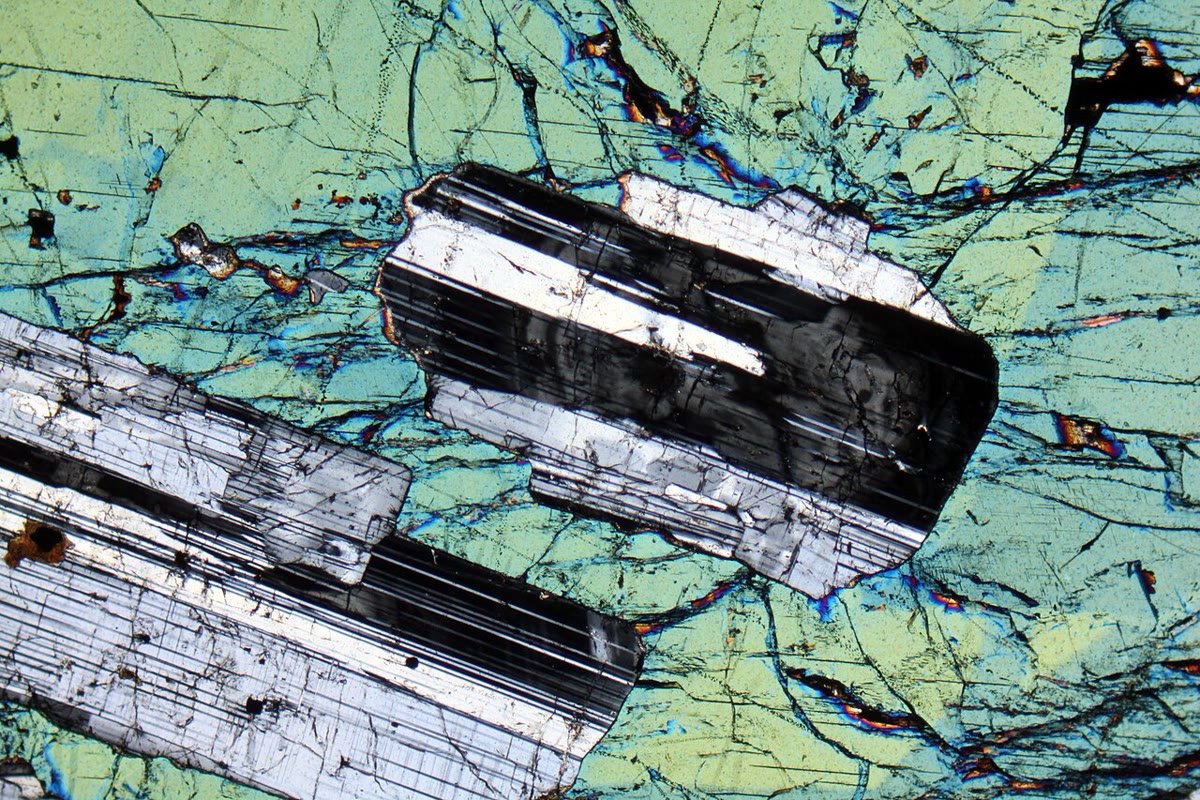
\includegraphics[height=4.6cm]{images/book4/b2-31-ophitic.jpg}\quad
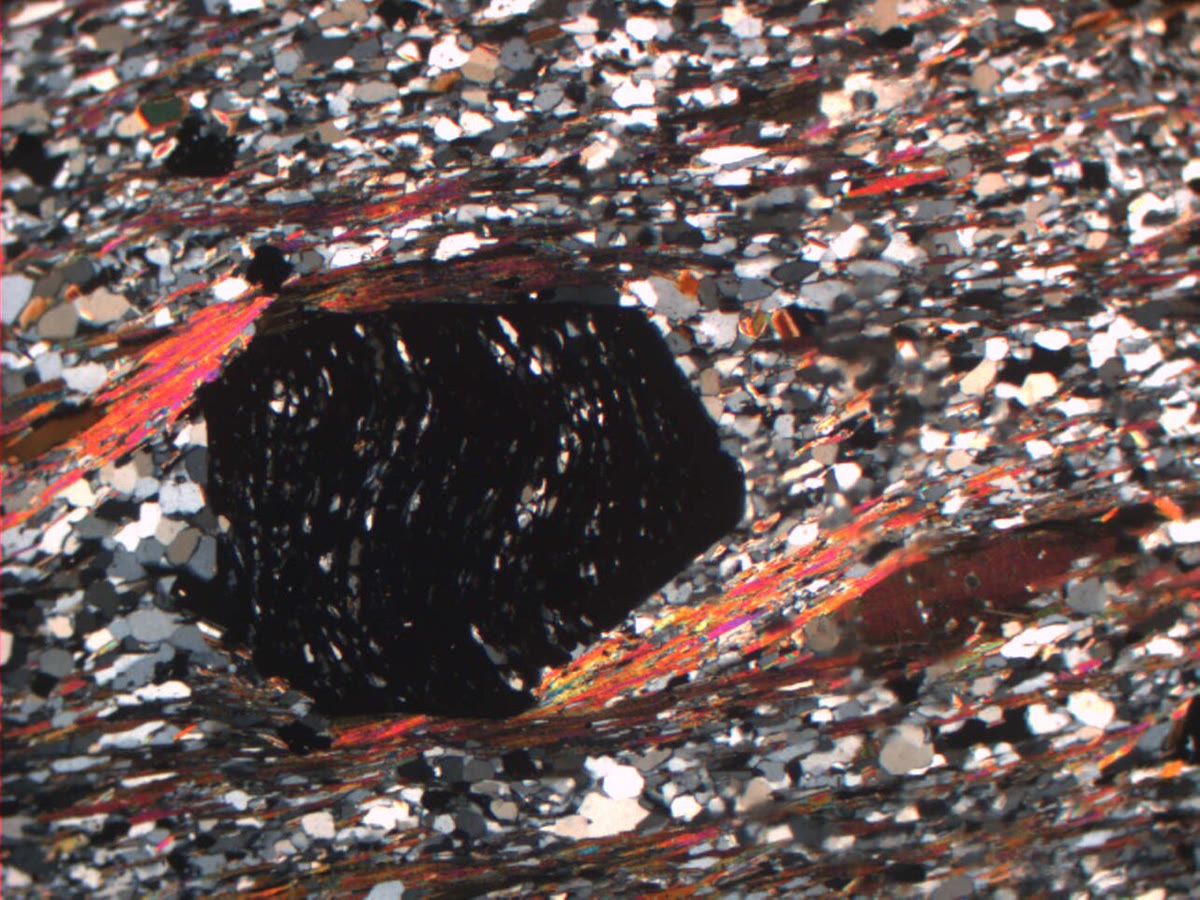
\includegraphics[height=4.6cm]{images/book4/b2-31-garnet-porphyroblast.jpg}
\par\smallskip{\small نسيجان بين مستقطِبين متقاطعين. يمينًا: بلّورة واحدة من الأوجيت (زرقاء
وخضراء) تحيط بصفائح من البلاجيوكلاز مخطّطة بتوأمتها، وهو ترتيب \omterm{def:b2:field-lab-methods-2:textures}{النسيج
الأوفيتي}؛ عرض حقل الرؤية \qty{7}{mm}. الصورة: \mbox{\textdir TLT Strekeisen, CC~BY-SA~4.0 (Wikimedia Commons)}.
يسارًا: شيست من الغارنت والميكا. والغارنت، الأسود لأنّه متماثل الخواصّ، بلّورة كبيرة
نمت في الحالة الصلبة؛ وتعبره محتبَسات من الكوارتز في مسارات، ويلتفّ حوله تورّق المسكوفيت
(بألوان زاهية) والبيوتيت (بنّي) والكوارتز (رمادي). الصورة:
\mbox{\textdir TLT Jackdann88, CC~BY~3.0 (Wikimedia Commons)}.}
\end{omfigure}
% ledger: photo:b2-31-ophitic, photo:b2-31-garnet

لا تنمو المعادن المتحوّلة كلّها بالوتيرة نفسها. فبعض الأنواع يطغى نموّها على غيرها فتصبح بلّورات كبيرة جدًّا،
تبتلع الحبيبات الصغيرة المحيطة بها في أثناء نموّها.

\begin{definition}[البورفيروبلاست، البويكيلوبلاست، مسار المحتبَسات، الهالة]\label{def:b2:field-lab-methods-2:porphyroblast}
\emph{البورفيروبلاست}\index{البورفيروبلاست} بلّورة كبيرة نمت في أثناء التحوّل
داخل أرضية أدقّ حبيبات؛ ويكوّنها الغارنت والستوروليت والكورديريت والكلوريتويد، من
مليمترات إلى عدّة سنتيمترات عرضًا. و\emph{البويكيلوبلاست}\index{البويكيلوبلاست}
بورفيروبلاست يحوي محتبَسات كثيرة من معادن أخرى. و\emph{مسار المحتبَسات}\index{مسار المحتبَسات}
خطّ من المحتبَسات المصطفّة داخل بورفيروبلاست، يحفظ
نسيج الأرضية في الوقت الذي طغت عليه البلّورة. و\emph{الهالة}\index{الهالة (نسيج تفاعلي)}
حافّة من معدن جديد واحد أو أكثر تحيط إحاطة تامّة بمعدن كان
يتفكّك، لأنّه لم يعد مستقرًّا مع
مجاوريه: إنّها نسيج تفاعلي، تجمّد قبل اكتمال التفاعل.
\end{definition}
% ledger: bgsM:textures, ouVM:textures

تأريخ نموّ \omterm{def:b2:field-lab-methods-2:porphyroblast}{البورفيروبلاست} نسبةً إلى التشوّه الذي صنع التورّق يكون بمقارنة \omterm{def:b2:field-lab-methods-2:porphyroblast}{مسار المحتبَسات}
($S_i$، النسيج الداخلي) بالتورّق خارج البلّورة ($S_e$، النسيج الخارجي). والمعايير الآتية، المرسومة في الشكل،
هي معايير مذكّرات التدريس المعتادة.
% ledger: ucsbH:inclusion-trails

\begin{method}[تأريخ بورفيروبلاست من مسارات محتبَساته]\label{met:b2:field-lab-methods-2:timing}
ابحث عن مقطع عمودي على التورّق، ثم قارن $S_i$ و$S_e$.
\begin{enumerate}
  \item \textbf{محتبَسات عشوائية}، و$S_e$ منحرف حول البلّورة: نمت قبل أن
        يتكوّن التورّق (\emph{سابقة للتكتونية}).
  \item \textbf{$S_i$ مستقيم مقطوع عند الحافّة}، غير متّصل بالنسيج $S_e$ المنحرف: نمت
        فوق تورّق أقدم، بين تشوّهين (\emph{بينية التكتونية}).
  \item \textbf{$S_i$ منحنٍ}، متّصل بالنسيج $S_e$: نمت في أثناء تكوّن التورّق، فدارت
        أو طُغي عليها في أثناء نموّها (\emph{متزامنة مع التكتونية}؛ وهو حلزون غارنت كرة الثلج).
  \item \textbf{$S_i$ مستقيم متّصل بنسيج $S_e$ غير منحرف}: نمت بعد التورّق
        (\emph{لاحقة للتكتونية}).
\end{enumerate}
\end{method}

\begin{omfigure}
\centering
\begin{tikzpicture}[x=1cm, y=1cm, font=\scriptsize]
% schematic after the criteria of ledger ucsbH:inclusion-trails
% panel 1: pre-tectonic
\begin{scope}[shift={(0,0)}]
\draw[omExo, line width=0.5pt] (-1.5,0.95) .. controls (-0.6,0.95) and (-0.5,0.85) .. (0,0.85) .. controls (0.5,0.85) and (0.6,0.95) .. (1.5,0.95);
\draw[omExo, line width=0.5pt] (-1.5,-0.95) .. controls (-0.6,-0.95) and (-0.5,-0.85) .. (0,-0.85) .. controls (0.5,-0.85) and (0.6,-0.95) .. (1.5,-0.95);
\draw[omExo, line width=0.5pt] (-1.5,0.45) .. controls (-0.9,0.45) and (-0.85,0.78) .. (0,0.78) .. controls (0.85,0.78) and (0.9,0.45) .. (1.5,0.45);
\draw[omExo, line width=0.5pt] (-1.5,-0.45) .. controls (-0.9,-0.45) and (-0.85,-0.78) .. (0,-0.78) .. controls (0.85,-0.78) and (0.9,-0.45) .. (1.5,-0.45);
\draw[omExo, line width=0.5pt] (-1.5,0) -- (-0.78,0); \draw[omExo, line width=0.5pt] (0.78,0) -- (1.5,0);
\filldraw[fill=omThm!15, draw=omThm, line width=0.6pt] (0,0) circle (0.72);
\draw[black, line width=0.7pt] (-0.4,0.2) -- (-0.25,0.35); \draw[black, line width=0.7pt] (0.1,0.35) -- (0.3,0.2);
\draw[black, line width=0.7pt] (-0.35,-0.2) -- (-0.15,-0.25); \draw[black, line width=0.7pt] (0.2,-0.15) -- (0.25,-0.4);
\draw[black, line width=0.7pt] (-0.05,0.05) -- (0.05,-0.1); \draw[black, line width=0.7pt] (0.35,0.0) -- (0.5,0.12);
\node at (0,-1.3) {سابق للتكتونية};
\end{scope}
% panel 2: inter-tectonic
\begin{scope}[shift={(3.4,0)}]
\draw[omExo, line width=0.5pt] (-1.5,0.95) .. controls (-0.6,0.95) and (-0.5,0.85) .. (0,0.85) .. controls (0.5,0.85) and (0.6,0.95) .. (1.5,0.95);
\draw[omExo, line width=0.5pt] (-1.5,-0.95) .. controls (-0.6,-0.95) and (-0.5,-0.85) .. (0,-0.85) .. controls (0.5,-0.85) and (0.6,-0.95) .. (1.5,-0.95);
\draw[omExo, line width=0.5pt] (-1.5,0.45) .. controls (-0.9,0.45) and (-0.85,0.78) .. (0,0.78) .. controls (0.85,0.78) and (0.9,0.45) .. (1.5,0.45);
\draw[omExo, line width=0.5pt] (-1.5,-0.45) .. controls (-0.9,-0.45) and (-0.85,-0.78) .. (0,-0.78) .. controls (0.85,-0.78) and (0.9,-0.45) .. (1.5,-0.45);
\draw[omExo, line width=0.5pt] (-1.5,0) -- (-0.78,0); \draw[omExo, line width=0.5pt] (0.78,0) -- (1.5,0);
\filldraw[fill=omThm!15, draw=omThm, line width=0.6pt] (0,0) circle (0.72);
\begin{scope}
\clip (0,0) circle (0.66);
\foreach \k in {-0.6,-0.3,0,0.3,0.6} {\draw[black, line width=0.7pt, dash pattern=on 2pt off 1.5pt] (-0.8,\k-0.45) -- (0.8,\k+0.45);}
\end{scope}
\node at (0,-1.3) {بيني التكتونية};
\end{scope}
% panel 3: syn-tectonic
\begin{scope}[shift={(6.8,0)}]
\draw[omExo, line width=0.5pt] (-1.5,0.8) -- (1.5,0.8);
\draw[omExo, line width=0.5pt] (-1.5,-0.8) -- (1.5,-0.8);
\draw[omExo, line width=0.5pt] (-1.5,0.4) -- (-0.6,0.4); \draw[omExo, line width=0.5pt] (0.6,0.4) -- (1.5,0.4);
\draw[omExo, line width=0.5pt] (-1.5,0) -- (-0.72,0); \draw[omExo, line width=0.5pt] (0.72,0) -- (1.5,0);
\draw[omExo, line width=0.5pt] (-1.5,-0.4) -- (-0.6,-0.4); \draw[omExo, line width=0.5pt] (0.6,-0.4) -- (1.5,-0.4);
\filldraw[fill=omThm!15, draw=omThm, line width=0.6pt] (0,0) circle (0.72);
\draw[black, line width=0.7pt, dash pattern=on 2pt off 1.5pt] (-0.6,0.4) .. controls (-0.35,0.4) and (-0.2,0.3) .. (-0.05,0.4) .. controls (0.1,0.5) and (0.35,0.4) .. (0.6,0.4);
\draw[black, line width=0.7pt, dash pattern=on 2pt off 1.5pt] (-0.72,0) .. controls (-0.3,0) and (-0.3,-0.45) .. (0,0) .. controls (0.3,0.45) and (0.3,0) .. (0.72,0);
\draw[black, line width=0.7pt, dash pattern=on 2pt off 1.5pt] (-0.6,-0.4) .. controls (-0.35,-0.4) and (-0.1,-0.5) .. (0.05,-0.4) .. controls (0.2,-0.3) and (0.35,-0.4) .. (0.6,-0.4);
\node at (0,-1.3) {متزامن مع التكتونية};
\end{scope}
% panel 4: post-tectonic
\begin{scope}[shift={(10.2,0)}]
\foreach \k in {-0.8,-0.4,0,0.4,0.8} {\draw[omExo, line width=0.5pt] (-1.5,\k) -- (1.5,\k);}
\filldraw[fill=omThm!15, draw=omThm, line width=0.6pt] (0,0) circle (0.72);
\begin{scope}
\clip (0,0) circle (0.66);
\foreach \k in {-0.8,-0.4,0,0.4,0.8} {\draw[black, line width=0.7pt, dash pattern=on 2pt off 1.5pt] (-0.8,\k) -- (0.8,\k);}
\end{scope}
\node at (0,-1.3) {لاحق للتكتونية};
\end{scope}
\end{tikzpicture}
\par\smallskip{\small مسارات المحتبَسات (بالأسود، متقطّعة) في بورفيروبلاست (بالأحمر) والتورّق
خارجه (بالرمادي)، في مقاطع عمودية على التورّق (رسم تخطيطي). من اليسار إلى اليمين:
محتبَسات نمت قبل التورّق، الذي ينحني حول البلّورة؛ ونسيج أقدم مستقيم مقطوع
عند الحافّة؛ ومسار ينحني ليلتحم بالتورّق، إذ دارت البلّورة في أثناء نموّها؛ ومسار
مستقيم يكمل التورّق غير المضطرب.}
\end{omfigure}

وعلم الصخور الوصفي كمّي أيضًا. فنسب معادن صخر ناري خشن الحبيبات
تسمّيه على \omterm{def:b2:magmatic-series:qapf}{مخطّط QAPF} (\cref{ch:b2:magmatic-series})، وهي تُقاس تحت
المجهر.

\begin{definition}[التحليل النمطي، عدّ النقاط]\label{def:b2:field-lab-methods-2:modal}
\emph{التحليل النمطي}\index{التحليل النمطي} هو قياس \omterm{def:b2:magmatic-series:qapf}{التركيب المعدني النمطي}
لصخر. وفي \emph{عدّ النقاط}\index{عدّ النقاط}، تُحرَّك شريحة
رقيقة تحت شعرتي التصالب في المجهر بخطوات متساوية على شبكة منتظمة، ويُسجَّل
المعدن الواقع تحت شعرتي التصالب عند كلّ نقطة؛ فنسبة النقاط التي
تقع على معدن تقدّر نسبته في الصخر.
\end{definition}

\begin{proposition}[ما يقيسه عدّ النقاط، وبأيّ جودة]\label{prop:b2:field-lab-methods-2:counting}
(أ) في صخر بلا اتجاه مفضّل، للكسر المساحي لمعدن في مقطع موضوع
عشوائيًا، في المتوسّط، قيمة كسره الحجمي. (ب) إذا وقعت $n$ نقطة باستقلال
على معدن كسره المساحي $p$، فإنّ النسبة المعدودة $\hat p = k/n$ متوسّطها $p$ وانحرافها
المعياري
\begin{equation}
\sigma = \sqrt{\frac{p(1-p)}{n}} , \qquad\text{أي إنّ}\qquad n = \frac{p(1-p)}{\sigma^2}
\label{eq:b2:field-lab-methods-2:binomial}
\end{equation}
نقطة لازمة لبلوغ انحراف معياري $\sigma$.
\end{proposition}

\begin{proof}
(أ) اقطع كتلة من الصخر ارتفاعها $H$ إلى مقاطع متوازية مساحة كلّ منها $S$. حجم
المعدن $\int_0^H a(z)\,\mathrm{d}z$، حيث $a(z)$ مساحته في المقطع عند الارتفاع $z$؛
وبالقسمة على الحجم $SH$، يكون الكسر الحجمي متوسّط الكسر المساحي $a(z)/S$ على
كلّ الارتفاعات، وهو القيمة المتوقّعة لارتفاع يُسحب عشوائيًا. (ب) تقع كلّ نقطة على
المعدن باحتمال $p$، مستقلّة عن غيرها، فيتبع عدد الإصابات $k$
التوزيع الحدّاني ذا الوسيطين $n$ و$p$، الذي متوسّطه $np$ وتباينه $np(1-p)$. والقسمة على
$n$ تعطي المتوسّط $p$ والتباين $p(1-p)/n$ للمقدار $\hat p$.
\end{proof}

يفترض برهان (ب) نقاطًا مستقلّة، وهو ما تقترب منه خطوة شبكة أكبر من
الحبيبات. فلمعدن يشكّل \qty{30}{\percent} من صخر، تعطي 500 نقطة $\sigma =
\sqrt{0.3 \times 0.7/500} = 0.020$، أي نقطتين مئويّتين؛ وبلوغ نقطة مئوية واحدة يتطلّب
$0.21/0.01^2 = 2100$ نقطة، أي أربعة أضعاف، لأنّ $\sigma$ لا تتناقص إلا بمعدّل $1/\sqrt n$. والخطأ
النسبي، $\sigma/p = \sqrt{(1-p)/(np)}$، أسوأ ما يكون للمعادن النادرة (الشكل أدناه،
يمينًا). ثم يُعاد حساب النسب المعدودة لتسمية الصخر: فتركيب نمطي فيه
\qty{10}{\percent} كوارتز، و30 فلسبار قلوي، و20 بلاجيوكلاز و40 معادن مافية يعطي Q وA
وP قدرها 16.7 و50.0 و33.3 حين تُردّ المكوّنات الفلسية الثلاثة إلى مجموع قدره 100. وعلى مثلّث
QAP يكون الصخر الذي تتراوح فيه Q بين 20 و60 غرانيتًا حين تقع نسبته \babelsublr{P/(A+P)} بين 10
و\qty{65}{\percent}: سيانوغرانيتًا دون 35، ومونزوغرانيتًا فوقها؛ ومن 65 إلى 90 يكون
غرانوديوريتًا، وفوق 90 توناليتًا. ومؤشّر اللون $M'$ هو نسبة المعادن الداكنة، أي
المعادن المافية وما يتّصل بها عدا المسكوفيت والأباتيت والكربونات الأوّلية؛ ويكون الصخر
فاتح اللون دون 35، ومتوسّط اللون من 35 إلى 65، وداكن اللون من 65 إلى 90.
% ledger: bgsI:qapf, bgsI:colour-index

\begin{omfigure}
\centering
\begin{minipage}[b]{0.49\linewidth}\centering
\begin{tikzpicture}
\begin{axis}[omrecord, width=0.96\linewidth, height=5.0cm, xmode=log, xmin=100, xmax=3000,
  ymin=0, ymax=45, xlabel={\foreignlanguage{arabic}{عدد النقاط المعدودة، $n$}}, ylabel={الخطأ النسبي $\sigma/p$ \babelsublr{(\unit{\percent})}},
  xtick={100,300,1000,3000}, xticklabels={100,300,1000,3000}, log ticks with fixed point,
  tick label style={font=\scriptsize}, label style={font=\small}]
% computed in figdata/bachelor-2/labmethods.py part pc (binomial counting)
\addplot[omThm, line width=1.1pt] table[x=n, y=rel05] {figdata/out/bachelor-2-labmethods-pc.dat};
\addplot[omProp, line width=1.1pt] table[x=n, y=rel20] {figdata/out/bachelor-2-labmethods-pc.dat};
\addplot[omDef, line width=1.1pt] table[x=n, y=rel50] {figdata/out/bachelor-2-labmethods-pc.dat};
\node[font=\scriptsize, text=omThm, anchor=south west] at (axis cs:330,24) {$p = 0.05$};
\node[font=\scriptsize, text=omProp, anchor=south west] at (axis cs:104,21.5) {$p = 0.2$};
\node[font=\scriptsize, text=omDef, anchor=south west] at (axis cs:104,10.3) {$p = 0.5$};
\end{axis}
\end{tikzpicture}
\end{minipage}\hfill
\begin{minipage}[b]{0.49\linewidth}\centering
\begin{tikzpicture}
\begin{axis}[omrecord, width=0.96\linewidth, height=5.0cm, xmin=52, xmax=76, ymin=-1.0, ymax=0.75,
  xlabel={قيمة \ce{SiO2} الموصى بها \babelsublr{(\unit{\percent})}}, ylabel={الفرق \babelsublr{(\unit{\percent})}},
  tick label style={font=\scriptsize}, label style={font=\small},
  ytick={-0.8,-0.4,0,0.4}, yticklabel style={/pgf/number format/fixed}]
% data: figdata/bachelor-2/labmethods.py part xrf; ledger: usgsT:sio2-table
\addplot[black!40, densely dotted] coordinates {(52,0) (76,0)};
\addplot[only marks, mark=*, mark size=1.5pt, omDef, error bars/.cd, y dir=both, y explicit]
  table[x=rec, y=diff, y error=s] {figdata/out/bachelor-2-labmethods-xrf.dat};
\node[font=\scriptsize, anchor=east] at (axis cs:73.0,-0.62) {RGM-1};
\node[font=\scriptsize, anchor=west] at (axis cs:56.6,0.40) {JA-2};
\node[font=\scriptsize, anchor=west] at (axis cs:60.8,-0.55) {AMH-1};
\node[font=\scriptsize, anchor=north] at (axis cs:54.1,-0.10) {BCR-2};
\end{axis}
\end{tikzpicture}
\end{minipage}
\par\smallskip{\small يمينًا: الخطأ المعياري النسبي لنسبة نمطية $p$ مقيسة \omterm{def:b2:field-lab-methods-2:modal}{بعدّ
النقاط}، \eqref{eq:b2:field-lab-methods-2:binomial}، لمعدن نادر وآخر شائع وثالث وفير.
يسارًا: صحّة قياس السيليكا بفلورة الأشعة السينية على خرزات مصهورة لعشر مواد مرجعية صخرية،
من البازلت إلى الغرانيت؛ وكلّ نقطة هي متوسّط 2 إلى 30 تحليلًا مطروحًا منه القيمة الموصى بها، مع
الانحراف المعياري للتحليلات شريطًا. البيانات: تاغارت وسيمز (2002)، هيئة المسح الجيولوجي الأمريكية.}
\end{omfigure}
% ledger: usgsT:sio2-table

\section{تحليل الصخر الكامل}\label{sec:b2:field-lab-methods-2:whole-rock}

يحتاج تحليل الصخر الكامل إلى عيّنة تمثّل الصخر: فورقة تعليمية من مجموعة الكيمياء الجيولوجية
لدى SERC تنصح بجمع عيّنة أكبر من أكبر حبيبة بعدّة مرّات،
تُسحق على مراحل وتُطحن إلى مسحوق ناعم. والأداة الأساسية للعناصر الرئيسية هي
فلورة الأشعة السينية. فحزمة من الأشعة السينية، تأتي عادةً من أنبوب بهدف من الروديوم، تطرد الإلكترونات
الداخلية من ذرّات العيّنة، فيصدر كلّ عنصر عندئذ أشعة سينية بطاقاته
المميِّزة الخاصّة (قانون موزلي، من كتب الفيزياء).
% ledger: sercX:xrf-scope

\begin{definition}[التحليل بفلورة الأشعة السينية، الخرزة المصهورة، الفقد عند الحرق]\label{def:b2:field-lab-methods-2:xrf}
\emph{التحليل بفلورة الأشعة السينية}\index{التحليل بفلورة الأشعة السينية} يقيس تراكيز
عناصر مادّة صلبة من شدّات الأشعة السينية المميِّزة التي تصدرها تحت حزمة من
الأشعة السينية، بالمقارنة مع معايير معروفة التركيب. و\emph{الخرزة
المصهورة}\index{الخرزة المصهورة} قرص زجاجي يُصنع بصهر مسحوق صخري موزون مع مادّة صاهرة موزونة،
مثل رباعي بورات الليثيوم، وصبّ المصهور؛ وهو متجانس أيًّا كانت حبيبات
المسحوق. و\emph{الفقد عند الحرق}\index{الفقد عند الحرق} هو كسر الكتلة الذي
يفقده مسحوق حين يُسخَّن عند درجة حرارة عالية ثابتة، ومعظمه ماء وثنائي أكسيد كربون يُطردان.
\end{definition}
% ledger: sercX:xrf-scope, usgsT:procedure

لا تتناسب شدّة خطّ مع وفرة عنصره إلا حين تتشابه العيّنات
والمعايير، لأنّ العناصر الأخرى تمتصّ الإشعاع وتعزّزه: وهذه آثار المصفوفة،
وآثار حجم الحبيبات، هي سبب صهر المسحوق في زجاج، وسبب تطبيق تصحيح
رياضي مع ذلك. وتقيس فلورة الأشعة السينية (XRF) العناصر الرئيسية العشرة، وفوق نحو \qty{1}{ppm}،
العناصر الأثرية مثل Rb وSr وZr وBa، بحدود كشف قدرها بضعة أجزاء في المليون. وهي
ضعيفة في العناصر الخفيفة (العدد الذري دون 11) ولا ترى النظائر ولا حالة
تأكسد الحديد.
% ledger: sercX:xrf-scope, usgsT:procedure

\begin{inthelab}[دفعة من الخرزات المصهورة]
في إجراء نشرته هيئة المسح الجيولوجي الأمريكية، يُسخَّن \qty{0.8000}{g} من مسحوق الصخر في
بوتقة من البلاتين والذهب عند \qty{925}{\celsius} مدّة 40 دقيقة، ويُبلَّغ عن فقد الكتلة بوصفه
\omterm{def:b2:field-lab-methods-2:xrf}{الفقد عند الحرق}. ويُضاف رباعي بورات الليثيوم، بقدر يترك \qty{8.0000}{g} بعد الصهر؛
وتوضع سبع بواتق في كلّ مرّة في فرن عند \qty{1120}{\celsius} وتُهزّ مدّة 35 دقيقة،
ثم تُصبّ في قوالب. وفي المطياف، يشعّع أنبوب روديوم ذو نافذة طرفية كلّ خرزة، وتُقارن
شدّات العناصر الرئيسية العشرة بشدّات المعايير. والتحليل الذي يقلّ مجموع
أكاسيده عن 97 أو يزيد على \qty{101}{\percent} يُعاد؛ ويُنجز المحلّل الواحد
نحو 250 عيّنة في الشهر.
\end{inthelab}
% ledger: usgsT:procedure

والمعايير نفسها صخور، حُلّلت مرّات كثيرة حتى صار تركيبها معروفًا بأفضل ممّا
يستطيع أيّ تحليل منفرد قياسه.

\begin{definition}[المادّة المرجعية الجيوكيميائية]\label{def:b2:field-lab-methods-2:rm}
\emph{المادّة المرجعية الجيوكيميائية}\index{المادّة المرجعية الجيوكيميائية} صخر طبيعي أو
معدن أو راسب، يُطحن ويُجانَس في دفعة كبيرة، ولتركيز واحد أو أكثر فيه
قيم راسخة أو مصدَّقة، ويُستعمل لمعايرة الأجهزة واختبار صحّة
طريقة.
\end{definition}
% ledger: usgsOFR:rm

بازلت BHVO-2 الصادر عن هيئة المسح الجيولوجي الأمريكية، الذي جُمع عام 1995 من حمم فاضت من فوهة هاليماوماو في
كيلاويا عام 1919، قيمة \ce{SiO2} الموصى بها له \qty{49.60}{\percent} وفيه \qty{394.1}{ppm} من
السترونشيوم. ويتحقّق المختبر من صحّته بقياس مثل هذه المواد كأنّها مجهولة، عند الطرف الأدنى
والأوسط والأعلى من مداه: ففي الشكل أعلاه، تسترجع طريقة الهيئة السيليكا ضمن
\qty{0.6}{\percent} من القيمة الموصى بها للصخور العشرة كلّها، من 54 إلى
\qty{74}{\percent} من \ce{SiO2}. وتحدّد عيّناته الفارغة حدوده: فحدّ الكشف يُؤخذ ثلاثة انحرافات
معيارية للعيّنات الفارغة المحضَّرة باستقلال، والحدّ الأدنى للإبلاغ خمسة، وكثيرًا ما تُقترح عشرة
لحدّ التقدير الكمّي.
% ledger: usgs:bhvo2-origin, usgs:bhvo2-major, usgs:bhvo2-trace, usgsOFR:rm, usgsOFR:lod, usgsT:sio2-table

\begin{method}[معايرة تحليل الصخر الكامل والتحقّق منه]\label{met:b2:field-lab-methods-2:calibration}
\begin{enumerate}
  \item \textbf{المعايرة.} قِس الشدّة $I$ لكلّ عنصر في خرزات عدّة مواد
        مرجعية، ووفّق خطّ المربّعات الصغرى $c = aI + b$ للتركيز الموصى به
        بدلالة الشدّة.
  \item \textbf{القياس.} حوّل شدّة كلّ عيّنة مجهولة إلى تركيز بواسطة الخطّ.
  \item \textbf{التحقّق.} قِس مادّة مرجعية كأنّها مجهولة في كلّ دفعة وقارنها
        بقيمتها الموصى بها؛ واجمع الأكاسيد \omterm{def:b2:field-lab-methods-2:xrf}{والفقد عند الحرق}، الذي ينبغي أن يقترب المجموع معه
        من \qty{100}{\percent}.
  \item \textbf{الإبلاغ.} قدّم التحليل كما قيس مع فقده عند الحرق؛ ولمخطّطات
        التصنيف، أعد حساب الأكاسيد إلى مجموع قدره 100 من دون المكوّنات المتطايرة.
\end{enumerate}
\end{method}

\section{تحليل المعادن: المسبار الإلكتروني الدقيق}\label{sec:b2:field-lab-methods-2:microprobe}

تعطي فلورة الأشعة السينية تركيب الصخر الكامل. أمّا تنطّق بورفيروبلاست من الغارنت، والتفاعلات
التي تسجّلها هالة، أو أزواج المعادن في مقياس حرارة جيولوجي، فتحتاج إلى تركيب حبيبة
مفردة، وتركيب نقاط داخلها.

\begin{definition}[المسبار الإلكتروني الدقيق، مطيافية تشتّت الطول الموجي]\label{def:b2:field-lab-methods-2:epma}
\emph{المسبار الإلكتروني الدقيق}\index{المسبار الإلكتروني الدقيق} جهاز يركّز حزمة من
الإلكترونات على بقعة من مقطع مصقول ويقيس الأشعة السينية المميِّزة الصادرة منها،
فيعطي تحليلًا كمّيًا لحجم عرضه بضعة ميكرومترات. وفي
\emph{مطيافية تشتّت الطول الموجي}\index{مطيافية تشتّت الطول الموجي}، تسقط الأشعة السينية
على بلّورة تحليلية لا تعكس إلى الكاشف إلا الطول الموجي الذي يحقّق قانون براغ عند
زاويتها؛ وتتحرّك البلّورة والكاشف معًا على دائرة (دائرة رولاند) لانتقاء خطّ كلّ
عنصر بدوره.
\end{definition}
% ledger: sercE:epma-spot, sercW:wds

قد تصغر البقع إلى 1 إلى \qty{2}{\micro\metre}، ويبلغ الكشف بضع عشرات من \unit{ppm}
كتليًا، للعناصر من البورون (العدد الذري 5) فما فوق. وتُقارن العدّات بعدّات
المعايير وتُصحَّح لآثار العدد الذري والامتصاص والفلورة (تصحيح ZAF). والمسبار
ذو المطيافات البلّورية الأربعة أو الخمسة يقيس من 10 إلى 12 عنصرًا في تحليل
واحد. ولا يستطيع كشف الهيدروجين ولا الهيليوم ولا الليثيوم، فيغيب ماء الميكا والأمفيبولات
عن مجاميعها؛ ولا يميّز الحديد الثنائي من الحديد الثلاثي؛ ويُبلغ عن أكاسيد، يُعاد منها
حساب الصيغة المعدنية كما في مجلّد السنة الأولى.
% ledger: sercE:epma-spot, sercE:epma-limits, sercW:wds

\begin{inthelab}[يوم على المسبار الإلكتروني الدقيق]
\begin{minipage}[t]{0.55\linewidth}\vspace{0pt}
الشرائح الرقيقة للمسبار مستطيلات في العادة أبعادها \mbox{\textdir TLT \qtyproduct{27 x 46}{mm}}، تُرقَّق إلى
\qty{30}{\micro\metre} وتُترك بلا غطاء زجاجي، ثم تُصقل صقلًا مستويًا. ومعظم السيليكات
عوازل كهربائية، فيُغطّى المقطع بغشاء موصل رقيق، أشيعه الكربون،
ليصرف شحنة الحزمة. ويعلّم المحلّل الحبيبات المراد قياسها على صور ملتقطة
تحت المجهر المستقطِب، ويحمّل المعايير مع المقاطع، ويترك الجهاز يمرّ
على قائمة من النقاط: مقطع عرضي من اللبّ إلى الحافّة عبر بلّورة غارنت، مثلًا.
\end{minipage}\hfill
\begin{minipage}[t]{0.42\linewidth}\vspace{0pt}
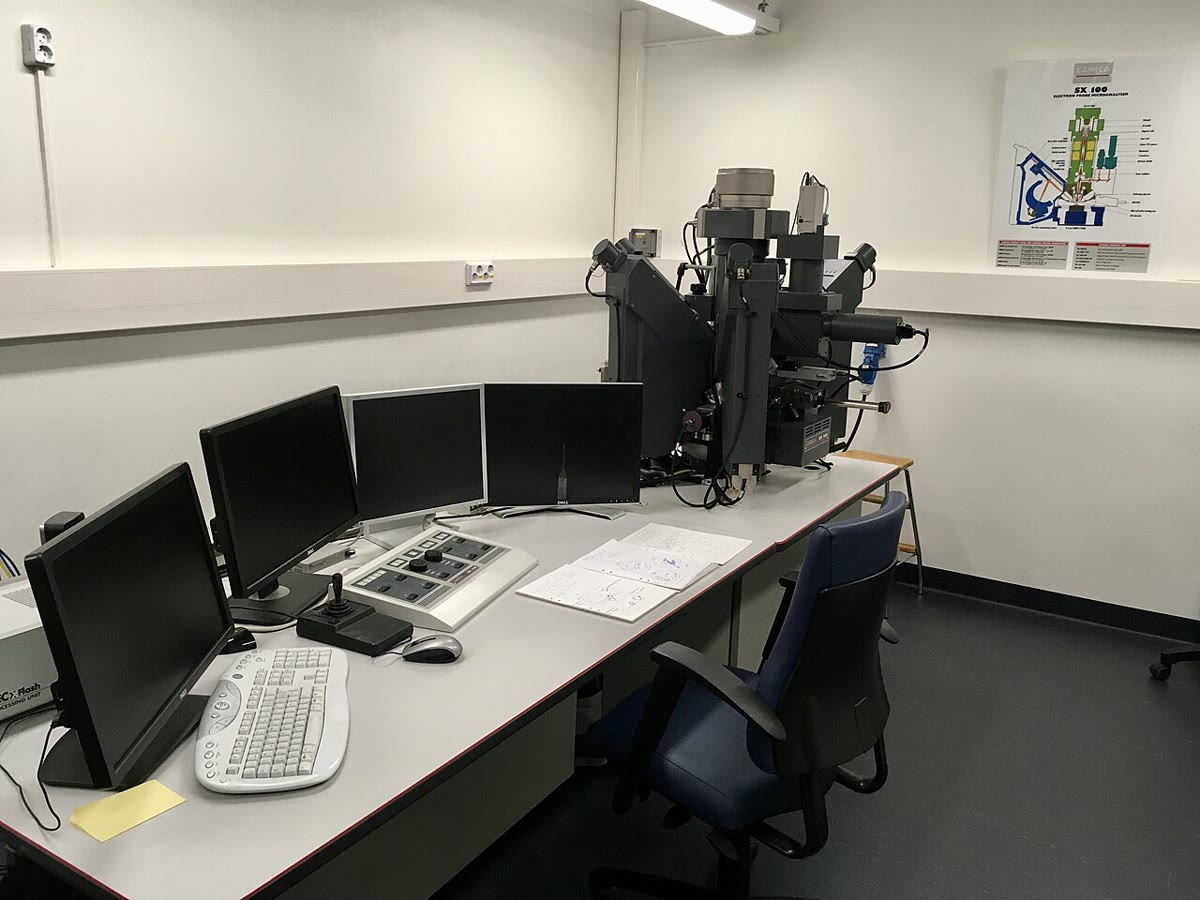
\includegraphics[width=\linewidth]{images/book4/b2-31-microprobe.jpg}
\par\smallskip{\scriptsize مسبار إلكتروني دقيق: العمود الإلكتروني، والمطيافات
حوله، ومكتب المشغّل. الصورة:\\\mbox{\textdir TLT Kallerna, CC~BY-SA~4.0 (Wikimedia Commons)}.}
\end{minipage}
\end{inthelab}
% ledger: sercE:epma-spot, sercE:coating, photo:b2-31-microprobe

\section{التحليل النظائري}\label{sec:b2:field-lab-methods-2:isotopes}

تستند المقتفيات النظائرية المشعّة المنشأ والأعمار (\cref{ch:b2:isotope-geochemistry}) إلى نسب مقيسة
بدقّة 0.01--\qty{0.001}{\percent}، لعناصر فُصلت عن الصخر بالإذابة
والكروماتوغرافيا بالتبادل الأيوني في مختبر نظيف، بهواء مرشَّح (من الفئة 100 إلى
1000 عادةً) حتى لا يضيف الغبار شيئًا إلى الكمّيات الصغيرة المحلَّلة.
% ledger: sercT:tims

\begin{definition}[مطيافية الكتلة بالتأيين الحراري، ICP-MS متعدّد المجمِّعات، الانحياز الكتلي]\label{def:b2:field-lab-methods-2:tims}
في \emph{مطيافية الكتلة بالتأيين الحراري}\index{مطيافية الكتلة بالتأيين الحراري} (TIMS)، يُحمَّل
عنصر منقّى على شريط معدني رقيق ويؤيَّن بتسخينه في الفراغ؛ وتُسرَّع الأيونات
عبر فرق جهد يصل إلى \qty{10}{kV}، وتُفصل بحسب الكتلة في قطاع مغناطيسي
وتُجمع. وفي \emph{ICP-MS متعدّد المجمِّعات}\index{ICP-MS متعدّد المجمِّعات} تأتي الأيونات من
بلازما مقترنة حثّيًا، تؤيّن العناصر العسيرة التأيين حراريًا، وتقيس عدّة
مجمِّعات حزم الكتل المختلفة في الوقت نفسه. و\emph{الانحياز
الكتلي}\index{الانحياز الكتلي} لقياس هو انحراف نسبة نظائرية مقيسة عن النسبة الحقيقية
للعيّنة، يسبّبه الجهاز الذي ينقل كتلة أو يؤيّنها بسهولة أكبر من
أخرى.
\end{definition}
% ledger: sercT:tims, sercM:mcicpms

يبلغ كلا الجهازين هذه الدقّة. يؤيّن TIMS عمومًا أقلّ من
\qty{1}{\percent} من الذرّات، ويتغيّر انحيازه الكتلي باستمرار في أثناء القياس. ويُصحَّح الانحياز بتثبيت نسبة نظيرين لا يغيّرها
أيّ تحلّل، وهذا يتطلّب عنصرًا له ثلاثة نظائر على الأقلّ، اثنان منها مستقرّان وغير
مشعّي المنشأ. وللسترونشيوم تُثبَّت $^{86}\mathrm{Sr}/^{88}\mathrm{Sr}$ عند 0.1194، وأحد الأشكال
الشائعة للتصحيح هو القانون الأسّي.
% ledger: sercT:tims, sercM:mcicpms, cheong14:mass-bias, ciaaw:sr-isotopes

\begin{proposition}[القانون الأسّي للانحياز الكتلي]\label{prop:b2:field-lab-methods-2:bias}
لنفترض أنّ كلّ نسبة مقيسة لنظيرين كتلتاهما $m_i$ و$m_j$ ترتبط بالنسبة
الحقيقية بالعلاقة $R_{ij}^{\mathrm{true}} = R_{ij}^{\mathrm{meas}}\,(m_i/m_j)^{\beta}$، مع أسّ واحد
$\beta$ للقياس كلّه. عندئذ تعطي النسبة المقيسة $r$ لزوج مرجعي، قيمته الحقيقية
$r_0$ معلومة،
\begin{equation}
\beta = \frac{\ln(r_0/r)}{\ln(m_k/m_l)}
\label{eq:b2:field-lab-methods-2:beta}
\end{equation}
للزوج المرجعي $k/l$، وتُصحَّح كلّ نسبة أخرى بالقيمة $\beta$ نفسها.
\end{proposition}

\begin{proof}
بتطبيق القانون على الزوج المرجعي يصير $r_0 = r\,(m_k/m_l)^\beta$؛ وبأخذ اللوغاريتمات،
$\ln(r_0/r) = \beta\ln(m_k/m_l)$، وهذه هي \eqref{eq:b2:field-lab-methods-2:beta}. والأسّ
مشترك بين كلّ نسب القياس بالفرض، فهو يصحّح كلًّا منها.
\end{proof}

وللسترونشيوم يكون الزوج المرجعي $^{86}\mathrm{Sr}/^{88}\mathrm{Sr}$ مع $r_0 = 0.1194$، وتكون
النسبة $^{87}\mathrm{Sr}/^{86}\mathrm{Sr}$ المصحَّحة هي النسبة المقيسة مضروبة في
$(m_{87}/m_{86})^\beta$. ووفرتا CIAAW، \qty{9.86}{\percent} من السترونشيوم 86
و\qty{82.58}{\percent} من السترونشيوم 88، تعطيان القيمة نفسها. وتقيس كلّ جلسة أيضًا معيارًا
نظائريًا مرجعيًا: فقد قاس أحد المختبرات \mbox{$^{87}\mathrm{Sr}/^{86}\mathrm{Sr} = 0.710252 \pm
0.000007$} على المادّة المرجعية NBS~987 في سبعة قياسات.
% ledger: cheong14:mass-bias, ciaaw:sr-isotopes

النسب وحدها لا تعطي تركيزًا. ولذلك تُمزج كمّية معلومة من \emph{مُضاف نظائري}، وهو محلول
للعنصر مُثرى اصطناعيًا بأحد نظائره، مع العيّنة المذابة قبل
الكيمياء، وتُقاس النسبة في المزيج. وتستعمله مختبرات TIMS لكلّ من
التراكيز ونسب الأمّ إلى البنت.
% ledger: sercT:tims

\begin{proposition}[التخفيف النظائري]\label{prop:b2:field-lab-methods-2:id}
لتحوِ عيّنة $N_x$ مولًا من نظير مرجعي $b$ ويحوِ مُضاف نظائري $N_s$ مولًا منه، ولتكن
$R_x$ و$R_s$ و$R_m$ نسب نظير ثانٍ $a$ إلى $b$ في العيّنة والمُضاف
والمزيج. عندئذ
\begin{equation}
N_x = N_s\,\frac{R_s - R_m}{R_m - R_x} .
\label{eq:b2:field-lab-methods-2:id}
\end{equation}
يُعطي خطأ نسبي $\varepsilon$ في $R_m$ للمقدار $N_x$ الخطأ النسبي $\mathcal{M}\varepsilon$،
مع معامل تضخيم الخطأ
\begin{equation}
\mathcal{M} = \frac{R_m\,(R_s - R_x)}{(R_s - R_m)(R_m - R_x)} ,
\label{eq:b2:field-lab-methods-2:mag}
\end{equation}
الذي يكون أصغر ما يمكن عندما $R_m = \sqrt{R_s R_x}$.
\end{proposition}
\index{التخفيف النظائري}

\begin{proof}
النظير $a$ محفوظ عند المزج: $R_m(N_x + N_s) = R_x N_x + R_s N_s$، فيكون $N_x(R_m - R_x) =
N_s(R_s - R_m)$، وهذه هي \eqref{eq:b2:field-lab-methods-2:id}. ومشتقّتها اللوغاريتمية
$\mathrm{d}\ln N_x/\mathrm{d}\ln R_m = R_m\,[-1/(R_s - R_m) - 1/(R_m - R_x)] = -\mathcal{M}$، مع
$\mathcal{M}$ كما في \eqref{eq:b2:field-lab-methods-2:mag}. وإلى حدّ الثابت الموجب $R_s - R_x$،
$1/\mathcal{M} = (R_s - R_m)(R_m - R_x)/R_m = R_s + R_x - R_m - R_sR_x/R_m$، ومشتقّته
$-1 + R_sR_x/R_m^2$ تنعدم عند $R_m = \sqrt{R_sR_x}$، وهي قيمة عظمى للمقدار $1/\mathcal{M}$.
\end{proof}

لا يحتاج \omterm{prop:b2:field-lab-methods-2:id}{التخفيف النظائري} إلى خطّ معايرة ولا إلى استرجاع كامل للعنصر عبر
الكيمياء: فما إن يُمزج المُضاف والعيّنة حتى تصيب الخسائر كليهما بالقدر نفسه. فمُضاف
منشور للسترونشيوم، مثلًا، يحوي \qty{99.65}{\percent} من السترونشيوم 84، مع
$^{84}\mathrm{Sr}/^{88}\mathrm{Sr} = 561.4$ و$^{86}\mathrm{Sr}/^{88}\mathrm{Sr} = 0.7661$، بتركيز
\qty{15.271}{\micro\gram} من السترونشيوم لكلّ غرام من المحلول. ونسبته 86/88 تبيّن لماذا لا يمكن
تصحيح \omterm{def:b2:field-lab-methods-2:tims}{الانحياز الكتلي} لمزيج مُضاف إليه بتثبيت $^{86}\mathrm{Sr}/^{88}\mathrm{Sr}$ عند
قيمتها الطبيعية: فالمُضاف قد غيّر تلك النسبة.
% ledger: cheong14:spike, cheong14:mass-bias

\section{حملة رسم خرائط على نافذة فاردن}\label{sec:b2:field-lab-methods-2:campaign}

في لبّ طيّة فاردن المحدّبة، قطع الحتّ الغطاء الرملي وكشف
القاعدة: شيست اخترقه غرانيت. والحملة التي ستزوّد المختبر تبدأ في
الحقل. يُقطع مساران من الغرب إلى الشرق عبر النافذة سيرًا على الأقدام، بمحطّة كلّ
\qty{100}{m}؛ ويُسجَّل الصنف الصخري عند كلّ منها، وتؤخذ عيّنات طازجة حيث يكون الصخر
غير مُجوًّى، تُرقَّم برقم المحطّة، وتُوجَّه حيث يُراد قياس الأنسجة. ويبيّن
الشكل ما تصادفه المحطّات: من المحطّات الثلاثين، عشر على الغرانيت، وعشر على الغطاء الرملي، وواحدة على
الشيست، وواحدة على الحجر الجيري وثمانٍ على رسوبيات قاع الوادي النهرية، حيث لا ينكشف
أيّ صخر.

\begin{omfigure}
\centering
\begin{tikzpicture}
\begin{axis}[axis equal image, xmin=2.4, xmax=4.6, ymin=3.1, ymax=5.0, width=0.66\linewidth,
  tick label style={font=\scriptsize}, xlabel={الشرق \babelsublr{(km)}}, ylabel={الشمال \babelsublr{(km)}},
  label style={font=\small}]
% units: figdata/shared/region.py (read only); stations: figdata/bachelor-2/labmethods.py part stations
\addplot[lith schist, draw=black, line width=0.3pt, even odd rule] table {figdata/out/shared-region-unit-schist.dat};
\addplot[lith granite, draw=black, line width=0.3pt, even odd rule] table {figdata/out/shared-region-unit-granite.dat};
\addplot[om lith={icsTriassic!35}{om sand}, draw=black, line width=0.3pt, even odd rule] table {figdata/out/shared-region-unit-sandstone.dat};
\addplot[om lith={icsJurassic!40}{om limestone}, draw=black, line width=0.3pt, even odd rule] table {figdata/out/shared-region-unit-limestone.dat};
\addplot[om lith={icsJurassic!15}{om shale}, draw=black, line width=0.3pt, even odd rule] table {figdata/out/shared-region-unit-shale.dat};
\addplot[lith alluvium, draw=black, line width=0.3pt, even odd rule] table {figdata/out/shared-region-unit-alluvium.dat};
\addplot[river] table {figdata/out/shared-region-river.dat};
\addplot[only marks, mark=*, mark size=1.6pt, mark options={fill=white, draw=black}]
  table[x=x_km, y=y_km] {figdata/out/bachelor-2-labmethods-stations.dat};
\addplot[only marks, mark=*, mark size=1.6pt, mark options={fill=omThm, draw=black},
  x filter/.expression={\thisrow{unit}==2 ? x : nan}]
  table[x=x_km, y=y_km] {figdata/out/bachelor-2-labmethods-stations.dat};
\node[font=\scriptsize, fill=white, inner sep=1pt, anchor=east] at (axis cs:2.76,3.7) {1};
\node[font=\scriptsize, fill=white, inner sep=1pt, anchor=west] at (axis cs:4.24,3.7) {15};
\node[font=\scriptsize, fill=white, inner sep=1pt, anchor=east] at (axis cs:2.76,4.4) {16};
\node[font=\scriptsize, fill=white, inner sep=1pt, anchor=west] at (axis cs:4.24,4.4) {30};
\draw[black, line width=0.5pt] (axis cs:3.5,4.44) -- (axis cs:3.5,4.62);
\node[font=\scriptsize, fill=white, inner sep=1pt, anchor=south] at (axis cs:3.5,4.62) {\foreignlanguage{arabic}{المحطّة \mbox{\textdir TLT 23}}};
\pic at (axis cs:4.45,4.75) {northarrow};
\end{axis}
\end{tikzpicture}
\par\smallskip{\small نافذة القاعدة في تلال فاردن مع المحطّات الثلاثين لمسارين من الغرب إلى الشرق،
يفصل بينهما \qty{100}{m}. النقاط الحمراء: محطّات على الغرانيت. الوردي مع الصلبان: الغرانيت؛ والرمادي: الشيست؛ والبنفسجي: الحجر
الرملي الترياسي؛ والأزرق: الحجر الجيري الجوراسي؛ والأزرق الفاتح: الطَّفل الجوراسي؛ والكريمي: رسوبيات النهر، الذي
يجري نحو الشرق. وعيّنة
الغرانيت في مسألة نهاية الأسبوع مأخوذة من المحطّة 23.}
\end{omfigure}

\begin{inthefield}[أخذ العيّنات للمختبر]
\centering
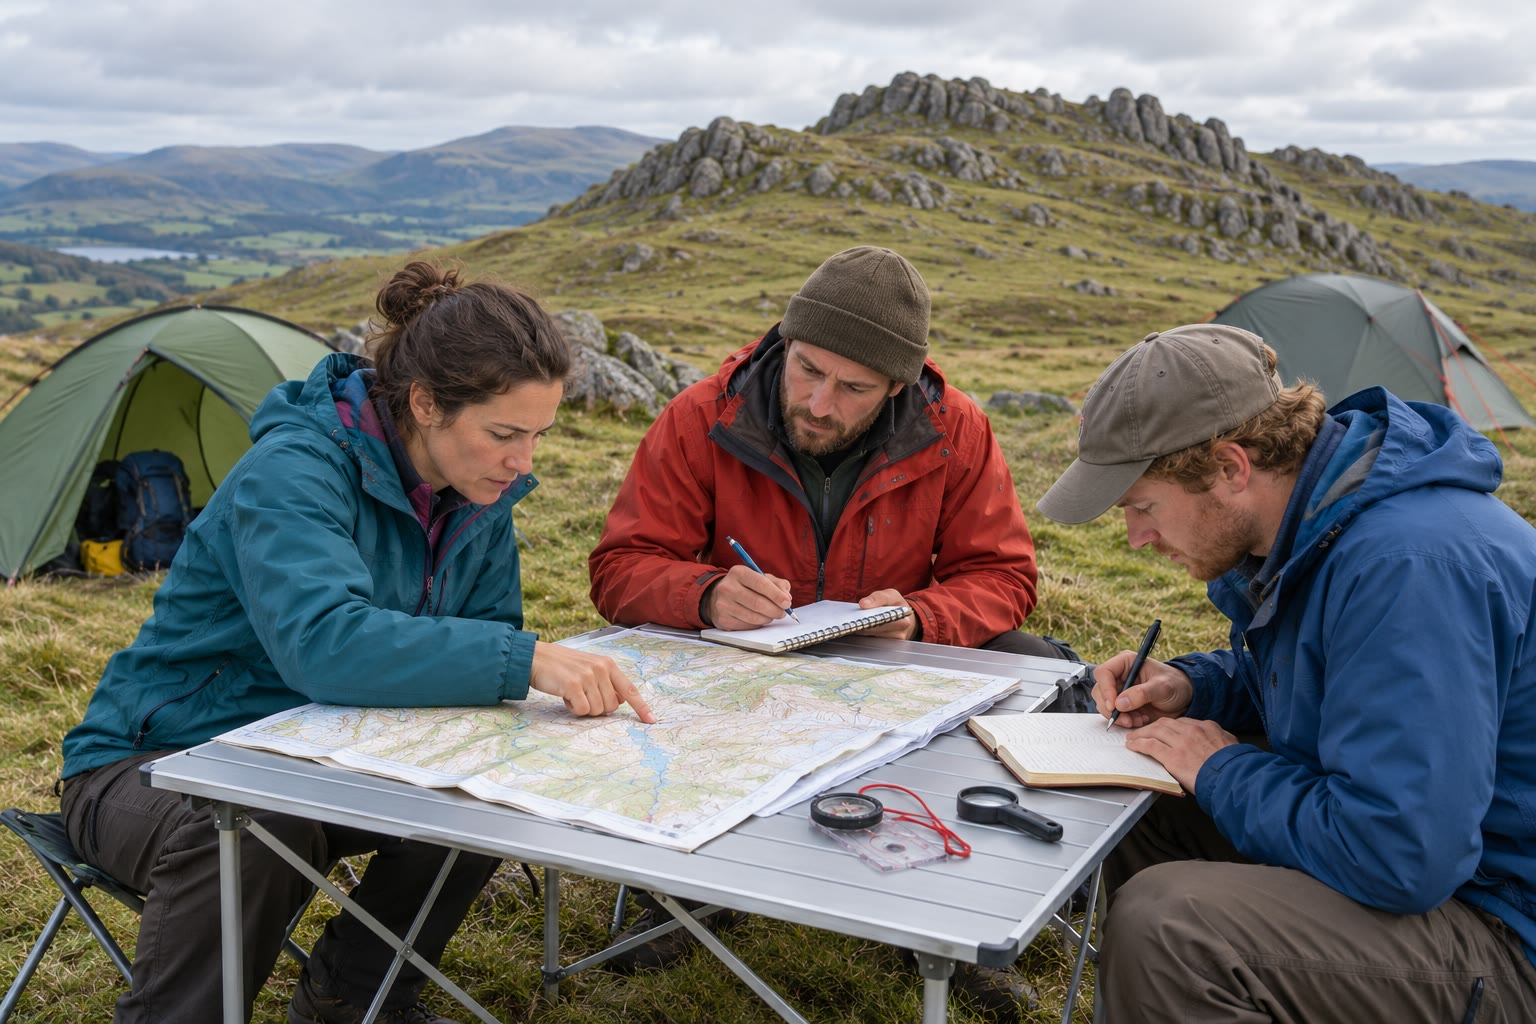
\includegraphics[width=0.56\linewidth]{images/book4/ai/b2-field-camp.jpg}
\par\smallskip{\small فريق ميداني يخطّط مسارات اليوم التالي (رسم توضيحي مولَّد بالذكاء الاصطناعي).}
\par\medskip\raggedright
في المساء ينقل الفريق المحطّات إلى الخريطة، ويتحقّق من أنّ لكلّ رقم عيّنة في
الدفاتر كيسًا يطابقه، ويقرّر أيّ العيّنات تذهب إلى أيّ مختبر. فعيّنة واحدة من كلّ صنف
تذهب إلى مختبر الشرائح الرقيقة؛ وأطزج عيّنات الغرانيت والشيست، أي أقلّها تجوية، تذهب
للسحق وتحليل الصخر الكامل؛ وتُنحّى بضع عيّنات من الغرانيت للنظائر. ويتبع
رقم المحطّة كلّ عيّنة عبر كلّ خطوة، من الكيس إلى الشريحة الرقيقة، فالمسحوق،
فالخرزة، فسطر في جدول بيانات، حتى يمكن تتبّع أيّ نتيجة شاذّة إلى
مكشفها.
\end{inthefield}

\section{جودة الرقم}\label{sec:b2:field-lab-methods-2:quality}

تضيف كلّ خطوة من السلسلة خطأها الخاصّ، وتُظهر طرائق هذا الفصل النوعين اللذين
تميّز بينهما كتب الكيمياء. فلعدّ النقاط وللنسب النظائرية أخطاء عشوائية في الغالب،
تتقلّص كلّما كبرت العدّات، بمعدّل $1/\sqrt n$؛ وللمعايرة أخطاء منهجية، لا يقلّلها
التكرار ولا تكشفها إلا مادّة مرجعية. ويُظهر شكل تحليلات السيليكا
كليهما: فالأشرطة هي دقّة الطريقة، والنقطة التي تبتعد عن الصفر بأضعاف كثيرة لشريطها
مقسومًا على الجذر التربيعي لعدد التحليلات تدلّ على انحياز. وقياس العنصر نفسه بطريقتين،
السترونشيوم بفلورة الأشعة السينية وبالتخفيف النظائري، تحقّق إضافي، لأنّ الطريقتين لا تشتركان في أيّ
معايرة. وتُعرض النتائج مع ارتيابها، مقرّبة إليه، ومع المواد المرجعية
التي قيست معها؛ والرقم الخالي منها لا يمكن مقارنته بأيّ رقم آخر.

\section*{التمارين}\label{sec:b2:field-lab-methods-2:exercises}

معطيات التمارين، ما لم يُذكر غير ذلك: الكتل الذرية H 1.008، وO 15.999، وMg 24.305، وAl
26.982، وSi 28.085، وK 39.098، وSr 87.62؛ وكتل النظائر $^{86}\mathrm{Sr}$ 85.909261،
و$^{87}\mathrm{Sr}$ 86.908878، و$^{88}\mathrm{Sr}$ 87.905612؛ والسترونشيوم الطبيعي
$^{84}\mathrm{Sr}/^{86}\mathrm{Sr} = 0.05680$، و\qty{9.86}{\percent} من $^{86}\mathrm{Sr}$؛ والمُضاف
الوارد في النصّ $^{84}\mathrm{Sr}/^{86}\mathrm{Sr} = 732.8$، و\qty{0.13599}{\percent} من
$^{86}\mathrm{Sr}$، والوزن الذرّي 83.9242، و\qty{15.271}{\micro\gram\per\gram}. قرّب إلى ثلاثة
أرقام معنوية ما لم يُذكر غير ذلك.
% ledger: ciaaw:H, ciaaw:O, ciaaw:Mg, ciaaw:Al, ciaaw:Si, ciaaw:K, ciaaw:sr-isotopes, cheong14:spike

\begin{exercise}[$\star$]\label{exo:b2:field-lab-methods-2:1}
(أ) سمِّ النسيج أو البلّورة: (1) دوليريت تحيط فيه بلّورات كبيرة من الأوجيت إحاطة تامّة بصفائح
البلاجيوكلاز؛ (2) رخام من حبيبات كالسيت متساوية الحجم تلتقي حدودها المستقيمة
ثلاثًا ثلاثًا؛ (3) بلّورة ستوروليت طولها \qty{5}{mm} مكتظّة بمحتبَسات الكوارتز في شيست ميكائي؛
(4) غارنت تحيط به حافّة متّصلة من البلاجيوكلاز والبيروكسين. (ب) تلتقي ثلاثة حدود حبيبية
بزوايا \ang{104} و\ang{128} و\ang{128}. أوجد نسبة توتّر الحدّ المقابل
للزاوية \ang{104} إلى توتّر كلّ من الحدّين الآخرين.
\end{exercise}

\begin{exercise}[$\star$]\label{exo:b2:field-lab-methods-2:2}
يحوي صخر خشن الحبيبات \qty{25}{\percent} كوارتز، و15 فلسبار قلوي، و40 بلاجيوكلاز، و12
بيوتيت و8 هورنبلند. (أ) أعد حساب Q وA وP. (ب) أوجد \babelsublr{P/(A+P)} وسمِّ الصخر. (ج) أوجد
مؤشّر لونه وصِفه.
\end{exercise}

\begin{exercise}[$\star$]\label{exo:b2:field-lab-methods-2:3}
يجد عدّ 800 نقطة معدنًا بنسبة \qty{12}{\percent}. (أ) أوجد الانحراف المعياري
لهذه النسبة، وقيمته النسبية. (ب) كم يكون مع 3200 نقطة؟
\end{exercise}

\begin{exercise}[$\star$]\label{exo:b2:field-lab-methods-2:4}
مسحوق كتلته \qty{0.8000}{g} يزن \qty{0.7712}{g} بعد الحرق، وتُصهر البقية مع
\qty{8.0000}{g} من المادّة الصاهرة. (أ) أوجد \omterm{def:b2:field-lab-methods-2:xrf}{الفقد عند الحرق}. (ب) أوجد الكسر الكتلي للعيّنة في
الخرزة. (ج) يحوي الزجاج \qty{5.20}{\percent} من \ce{SiO2}. أوجد سيليكا المسحوق المحروق
وسيليكا المسحوق الأصلي.
\end{exercise}

\begin{exercise}[$\star\star$]\label{exo:b2:field-lab-methods-2:5}
(أ) كم نقطة تلزم لقياس معدن ثانوي يشكّل \qty{2}{\percent} من صخر
بخطأ معياري نسبي قدره \qty{10}{\percent}؟ (ب) وكم لمعدن يشكّل \qty{30}{\percent}،
بالخطأ النسبي نفسه؟ (ج) علّق على الجهد الذي يتطلّبه معدن نادر.
\end{exercise}

\begin{exercise}[$\star\star$]\label{exo:b2:field-lab-methods-2:6}
في نتائج هيئة المسح الجيولوجي الأمريكية الواردة في الشكل، أعطى الريوليت RGM-1 القيمة \mbox{\textdir TLT \ce{SiO2} $= 72.89$} بانحراف
معياري 0.19 في 20 تحليلًا (الموصى بها 73.45)، وأعطى البازلت BCR-2 القيمة 54.17 بانحراف 0.13 في
20 تحليلًا (الموصى بها 54.1). (أ) أوجد نسبة الاسترجاع لكلّ منهما، بالمئة. (ب) أوجد الانحراف
المعياري لكلّ متوسّط، وعبّر عن كلّ فرق عن القيمة الموصى بها بوحدات منه.
(ج) أيّ النتيجتين تُظهر انحيازًا؟ وهل الطريقة أقلّ دقّة في RGM-1؟
\end{exercise}

\begin{exercise}[$\star\star$]\label{exo:b2:field-lab-methods-2:7}
يُراد التحقّق من تحليل \omterm{def:b2:field-lab-methods-2:epma}{بالمسبار الإلكتروني الدقيق} لفلوغوبيت نقيّ، $\mathrm{KMg_3AlSi_3O_{10}(OH)_2}$.
(أ) أوجد الكتلة المولية للصيغة والكسر الكتلي لماء \ce{H2O} الذي تحويه. (ب) أوجد
الكسور الكتلية لأكاسيد \ce{K2O} و\ce{MgO} و\ce{Al2O3} و\ce{SiO2}، والمجموع الذي يعطيه
تحليل دقيق. (ج) لماذا لا يكون مجموع قدره نحو \qty{96}{\percent} لميكا تحليلًا سيّئًا؟
\end{exercise}

\begin{exercise}[$\star\star$]\label{exo:b2:field-lab-methods-2:8}
يعطي قياس TIMS على معيار للسترونشيوم $^{86}\mathrm{Sr}/^{88}\mathrm{Sr} = 0.11905$
و$^{87}\mathrm{Sr}/^{86}\mathrm{Sr} = 0.71062$. (أ) أوجد الأسّ $\beta$ للقانون الأسّي.
(ب) صحّح النسبة $^{87}\mathrm{Sr}/^{86}\mathrm{Sr}$، إلى خمسة منازل عشرية. (ج) هل فُضِّل النظير الخفيف أم
الثقيل في القياس؟
\end{exercise}

\begin{exercise}[$\star\star$]\label{exo:b2:field-lab-methods-2:9}
للتحقّق من تخفيفه النظائري، يضيف مختبر إلى \qty{0.0500}{g} من البازلت المرجعي BHVO-2
\qty{0.1000}{g} من المُضاف الوارد في النصّ، ويقيس $^{84}\mathrm{Sr}/^{86}\mathrm{Sr} =
0.874$ في المزيج. (أ) أوجد عدد مولات $^{86}\mathrm{Sr}$ في جزء المُضاف. (ب) أوجد
عدد مولات $^{86}\mathrm{Sr}$ في العيّنة، وتركيز السترونشيوم فيها بوحدة \unit{ppm}. (ج) قارن بالقيمة
الموصى بها \qty{394.1}{ppm}.
\end{exercise}

\begin{exercise}[$\star\star\star$]\label{exo:b2:field-lab-methods-2:10}
لمُضاف السترونشيوم الوارد في النصّ ($R_s = 732.8$، $R_x = 0.05680$): (أ) أوجد نسبة المزيج
التي تجعل تضخيم الخطأ أصغر ما يمكن، وقيمته عندها؛ (ب) احسب $\mathcal M$ عند
$R_m = 0.1$ و0.5 و1.664 و100؛ (ج) اشرح لماذا ينبغي تجنّب مزيج قريب من أيّ من العضوين الطرفيين،
وما مقدار الحرّية المتاحة للمحلّل عمليًا.
\end{exercise}

\begin{exercise}[$\star\star\star$]\label{exo:b2:field-lab-methods-2:11}
يجد عدّ في غرانيت 400 نقطة على الفلسبار، \qty{62}{\percent} منها بلاجيوكلاز. (أ) بمعاملة
البلاجيوكلاز بين نقاط الفلسبار عدًّا حدّانيًا، أوجد الانحراف المعياري للنسبة
\babelsublr{P/(A+P)}. (ب) كم تبعد النتيجة عن حدّ الغرانوديوريت، بالانحرافات المعيارية؟ (ج) كم
نقطة فلسبار تضعها على بعد انحرافين معياريين من الحدّ؟
\end{exercise}

\begin{exercise}[$\star\star\star$]\label{exo:b2:field-lab-methods-2:12}
يشغل معدن كسرًا $p$ من صخر. (أ) بيّن أنّ احتمال أن تخطئه $n$ نقطة مستقلّة
جميعًا هو $(1-p)^n$. (ب) كم نقطة تعطي فرصة لا تقلّ عن \qty{95}{\percent} لإصابة
معدن يشكّل \qty{1}{\percent} من الصخر مرّة واحدة على الأقلّ؟ (ج) الأمر نفسه للزركون عند
\qty{0.05}{\percent}، واستنتج كيف ينبغي البحث عن معدن ثانوي.
\end{exercise}

\section*{مسألة نهاية الأسبوع}

\begin{problem}[{مسألة نهاية الأسبوع --- من المكشف إلى التحليل}]\label{pb:b2:field-lab-methods-2:1}
% invented sample; data: ledger rows below; values: calc/ch31.py
أُخذت العيّنة VH-23 من غرانيت فاردن عند المحطّة 23 من الحملة. وعُدّت نقاط شريحة رقيقة
منها على شبكة منتظمة من 1200 نقطة: الكوارتز 372، والفلسبار القلوي 348، والبلاجيوكلاز 324،
والبيوتيت 108، والمسكوفيت 36، والأكاسيد المعتمة 12. وصار مسحوق كتلته \qty{0.8000}{g} يزن \qty{0.7949}{g}
بعد الحرق عند \qty{925}{\celsius} وصُهر مع \qty{8.0000}{g} من المادّة الصاهرة. وأعطت خرزات ثلاث
مواد مرجعية شدّات \ce{SiO2} الآتية (بوحدة \unit{kcps}، أي بآلاف العدّات في الثانية): للمادّة BCR-2، وقيمتها
الموصى بها \qty{54.1}{\percent}، الشدّة 21.66؛ وللمادّة AGV-2، وقيمتها 59.3، الشدّة 23.70؛ وللمادّة RGM-1، وقيمتها 73.45، الشدّة 29.37؛ وأعطت خرزة الغرانيت
28.63. ومجموع أكاسيد الغرانيت الأخرى \qty{27.15}{\percent}. وللنظائر،
أُذيب \qty{0.1000}{g} من المسحوق ومُزج مع \qty{0.2500}{g} من المُضاف الوارد في النصّ؛
وتُعدّ العيّنة ذات وفرات السترونشيوم الطبيعية الواردة في التمارين. استعمل معطيات
التمارين.

\noindent\textbf{الجزء الأول --- التركيب النمطي.}
\begin{enumerate}
  \item أوجد النسبة النمطية لكلّ معدن.
  \item أوجد الانحراف المعياري لنسبة الكوارتز، والانحراف المعياري النسبي
        لنسبة المسكوفيت.
  \item أوجد $M$ ومؤشّر اللون $M'$، وصِف الصخر.
  \item أعد حساب Q وA وP إلى مجموع قدره 100.
  \item أوجد \babelsublr{P/(A+P)} وسمِّ الصخر على \omterm{def:b2:magmatic-series:qapf}{مخطّط QAPF}.
  \item مع الانحراف المعياري الحدّاني للنسبة \babelsublr{P/(A+P)} على نقاط الفلسبار البالغ عددها 672، هل التسمية
        مؤكّدة؟
  \item كم نقطة تجعل الانحراف المعياري لنسبة الكوارتز نقطة مئوية
        واحدة؟
\end{enumerate}

\noindent\textbf{الجزء الثاني --- السيليكا بفلورة الأشعة السينية.}
\begin{enumerate}[resume]
  \item أوجد \omterm{def:b2:field-lab-methods-2:xrf}{الفقد عند الحرق}.
  \item أوجد الكسر الكتلي للعيّنة في الخرزة، وسيليكا الزجاج إذا كان
        المسحوق المحروق يحوي \qty{72}{\percent}.
  \item وفّق خطّ المربّعات الصغرى $c = aI + b$ عبر المواد المرجعية الثلاث؛ وأعطِ $a$ إلى
        أربعة منازل عشرية و$b$ إلى منزلتين.
  \item أوجد نسبة \ce{SiO2} في الغرانيت، إلى منزلتين عشريتين.
  \item أوجد البواقي للمواد المرجعية الثلاث. هل الخطّ ملائم؟
  \item اجمع الأكاسيد \omterm{def:b2:field-lab-methods-2:xrf}{والفقد عند الحرق}. هل يعيد إجراء هيئة المسح الجيولوجي الأمريكية هذا التحليل؟
  \item أعد حساب السيليكا إلى مجموع قدره 100 من دون المكوّنات المتطايرة.
\end{enumerate}

\noindent\textbf{الجزء الثالث --- \omterm{def:b2:field-lab-methods-2:tims}{الانحياز الكتلي}.}
\begin{enumerate}[resume]
  \item من وفرات CIAAW، أوجد النسبة الطبيعية $^{86}\mathrm{Sr}/^{88}\mathrm{Sr}$ وقارنها
        بالقيمة المستعملة للتطبيع.
  \item يعطي جزء غير مُضاف إليه $^{86}\mathrm{Sr}/^{88}\mathrm{Sr} = 0.11853$. أوجد $\beta$ إلى
        أربعة منازل عشرية.
  \item ويعطي $^{87}\mathrm{Sr}/^{86}\mathrm{Sr} = 0.71655$. صحّحها، إلى خمسة منازل عشرية.
  \item أوجد الانحياز لكلّ وحدة كتلة، بالمئة.
  \item لماذا لا يمكن إجراء هذا التصحيح على المزيج المُضاف إليه في الجزء الرابع؟
\end{enumerate}

\noindent\textbf{الجزء الرابع --- \omterm{prop:b2:field-lab-methods-2:id}{التخفيف النظائري}.}
\begin{enumerate}[resume]
  \item تحقّق من أنّ المُضاف يحوي \qty{99.65}{\percent} من السترونشيوم 84 و\qty{0.13599}{\percent}
        من السترونشيوم 86.
  \item أوجد عدد مولات السترونشيوم ومولات $^{86}\mathrm{Sr}$ في جزء المُضاف، إلى أربعة
        أرقام معنوية.
  \item تحقّق من القيمتين $R_s = 732.8$ و$R_x = 0.05680$ الواردتين في التمارين.
  \item النسبة المصحَّحة للمزيج $R_m = 1.6812$. أوجد عدد مولات $^{86}\mathrm{Sr}$
        في العيّنة.
  \item أوجد تضخيم الخطأ. ومع معرفة $R_m$ بدقّة \qty{0.01}{\percent} وتركيز
        المُضاف بدقّة $\pm\qty{0.031}{\micro\gram\per\gram}$، أوجد الارتياب النسبي في
        النتيجة.
  \item أوجد تركيز السترونشيوم في غرانيت فاردن، بوحدة \unit{ppm}.
\end{enumerate}
\end{problem}
% ledger: bgsI:qapf, bgsI:colour-index, usgsT:procedure, usgsT:sio2-table, ciaaw:sr-isotopes, cheong14:spike, cheong14:mass-bias
